\chapter{The switching model of viscosity}
\label{chp:switching_model}

\graphicspath{{images/development_of_switching_model/}}

In this chapter I initially explore the effect of resolution on the Braginskii model of viscosity. A direct numerical implementation of the tensor as written in~\eqref{eq:brag_new} fails to capture the transition between isotropic and anisotropic viscosity in the vicinity of magnetic null points when such an implementation is used in simulations performed at resolutions typical of modern 3D simulations. This motivates the implementation of a different model of viscosity, the switching model, which approximates the Braginskii tensor as an interpolation between fully-isotropic and fully-parallel tensors. Three potential interpolation (or switching) functions are introduced: a phenomenological model derived from considering the probability of momentum transport in different magnetic field strengths, and two functions based on coefficients of the full Braginskii tensor. The development of the first function, referred to here as the von Mises switching function can be found in~\cite{mactaggartBraginskiiMagnetohydrodynamicsArbitrary2017}. Finally, I present the results of a suite of simulations performed at various resolutions which illustrate the differences between the models and are used to gauge their efficacy.

\section{The transition from isotropic to anisotropic in the full Braginskii tensor}

In strong magnetic fields, the Braginskii tensor can be approximated by the parallel term~\eqref{eq:braginskii_parallel_term} while in the absence of a magnetic field, the tensor reduces to that of isotropic viscosity~\eqref{eq:isotropic_viscous_tensor}. Between these extremes the perpendicular and drift components of the tensor can become relevant~\cite{erdelyiResonantAbsorptionAlfven1995a}. The form of the Braginskii tensor as written in~\eqref{eq:brag_new} is nearly in a form useful in understanding how quickly the tensor transitions from isotropic to anisotropic with changing magnetic field strength, since the isotropic component is completely isolated. Similarly, the parallel component can be isolated by further rewriting the tensor as,
\begin{equation}
\begin{split}
\ten{\sigma}_{\rm brag} &= \frac{3\eta_0+\eta_1-4\eta_2}{3}\ten{W}^{(0)}\\
& + (\eta_2-\eta_1)[\ten{W}(\vec{b}\otimes\vec{b})+(\vec{b}\otimes\vec{b})\ten{W} - \frac{2}{3}(\ten{W}\vec{b}\cdot\vec{b})\ten{I}] \\
& + \eta_1\ten{W},
\end{split}
\label{eq:brag_new2}
\end{equation}

\begin{figure}[t]
  \centering
  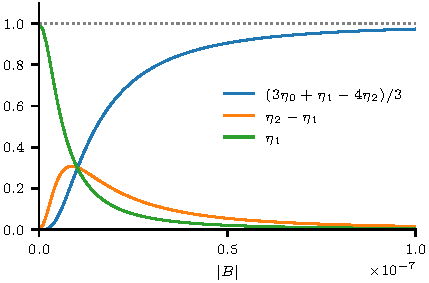
\includegraphics[width=0.5\linewidth]{brag_coeffs_2.pdf}
  \mycaption{Coefficients of the terms in the Braginskii tensor~\eqref{eq:brag_new2} normalised against $\eta_0$.}{In these plots, $\alpha = 10^{8}$, a value realistic of the corona.}%
  \label{fig:brag_coeffs2}
\end{figure}

Figure~\ref{fig:brag_coeffs2} presents the magnitudes of the coefficients of each of the terms in tensor~\eqref{eq:brag_new2} where $\alpha = e\tau/m = 10^{8}$ (recall that the coefficients $\eta_1$ and $\eta_2$ are defined in terms of the quantity $x = \omega \tau =\alpha |\vec{B}|$). Over the extremely small range between $|\vec{B}| = 0$ T and $10^{-7}$ T, the Braginskii tensor goes from completely isotropic to nearly completely parallel. Over the same range the coefficient corresponding to the perpendicular viscosity becomes relatively significant before tending to zero for large $|\vec{B}|$. The small transition region presents a problem in the numerical simulation of anisotropic viscosity, where the magnetic field strength likely changes more rapidly in space than can be captured by the coefficients in~\eqref{eq:brag_new2} when applied on a discretised grid. This is illustrated by an example.

In the simulations of magnetic null points found later in section~\ref{sec:slow_null_point}, the magnetic field strength changes linearly in the $x$-direction. Given a typical grid spacing of $\Delta x = 0.01$, the jump in magnetic field from one grid point to the next is $5\times 10^{-5}$ T. This is much greater than the range over which the Braginskii tensor transitions between isotropic and anisotropic regimes and the viscous response is under-resolved as a result. For these simulations, the resolution would have to increase by a factor of $100$ per dimension to even begin to resolve the region of transition. This region may be physically significant, particularly in magnetic configurations involving large-scale weak field, for example in fragmented current sheets located at null points~\cite{wyperNonlinearTearing3D2014} and in the heliospheric current sheet where field strengths are estimated to be on the order of $10^{-10}$ T~\cite{czechowskiStructureHeliosphericCurrent2010}. Given the abundance of observable null points and their involvement in high-energy phenomena, it is possible that the isotropic (and perpendicular) viscosity regions in the vicinity of a null point plays an important part in its dynamics, hence it is important to be able to properly resolve these regions and investigate their physical relevance. At the resolutions typically studied in general 3D MHD simulations (between $300$ and $1000$ grid points per dimension) the isotropic regions in the vicinity of null points would be poorly resolved, were the full Braginskii tensor to be employed. This is particularly true in simulations where null points are not the main focus of the simulation, but are dynamically created by some process.

Computational solutions such as refining the mesh near the null or implementing a multigrid method may help to improve the resolution of a given simulation and better resolve the viscosity transition region, however such approaches can be complex to implement in existing codes. An alternative to improving the resolution itself is to artificially scale $|\vec{B}|$ in the expression for the parallel Braginskii transport parameter~\eqref{eq:perp_visc_coeff} in order to enlarge the isotropic region to resolvable scales. This is done by artificially setting $\alpha$ in the argument $x$ of the parallel and perpendicular coefficients in~\eqref{eq:perp_visc_coeff} and~\eqref{eq:drift_visc_coeff} to a value other than its physical value.

Consider the effect of decreasing $\alpha$ on the coefficients shown in figure~\ref{fig:brag_coeffs2}. Decreasing $\alpha$ exaggerates the size of the region near $|\vec{B}| = 0$ where the isotropic and perpendicular components are significant. In this way, $\alpha$ can be used as a controllable parameter to prescribe the size of the region of isotropic (or perpendicular) viscosity around a null point.

As well as exaggerating the region of isotropic viscosity, this approach requires exaggerating the region of perpendicular viscosity. To see this, consider the contributions to the field-aligned component of~\eqref{eq:brag_new2} in a coordinate system where the field lies in the $z$-direction,
\begin{equation}
  \label{eq:z_aligned_field}
(\sigma_{brag})_{zz} = \frac{3\eta_0+\eta_1-4\eta_2}{3} W_{zz} + (\eta_2 - \eta_1) \frac{4}{3} W_{zz} + \eta_1 W_{zz} = \eta_0 W_{zz}.
\end{equation}
If the coefficient of the perpendicular component $\eta_2 - \eta_1$ is not scaled identically to the isotropic and parallel coefficients, the terms in~\eqref{eq:z_aligned_field} no longer cancel appropriately and the field-aligned momentum transport is no longer independent of $|\vec{B}|$ (as it should be in models of anisotropic viscosity). Hence, scaling the coefficients in the Braginskii tensor to enlarge the isotropic region necessarily requires also scaling the size of the perpendicular region. While this may be a useful feature, creating a purely parallel-isotropic switching model offers an alternative which avoids the inclusion of perpendicular viscosity altogether.


\section{The switching model}

The switching model is a model of viscosity that approximates the full Braginskii tensor throughout most of the solar corona. By stripping out the perpendicular and drift components of the full Braginskii tensor, the model presents a cleaner, better-resolved model of anisotropic viscosity. It focuses on what are, in most cases, the physically important parts of anisotropic viscosity in the solar corona: the parallel and isotropic components. The idea at the core of the model is the interpolation between the parallel and isotropic tensors, approximating the way in which the Braginskii tensor changes between strong and weak fields.

For a general interpolation function $\tilde{s}(|\vec{B}|)$, henceforth referred to as a switching function, the switching model takes the form,
\begin{equation}
  \label{eq:switching_model_simple}
\ten{\sigma}_{\text{swi}} = \eta_0 \left( 1 - \tilde{s} \right) \ten{W} + \eta_0 \tilde{s} \ten{W}^{(0)},
\end{equation}
or,
\begin{equation}
  \label{eq:switching_model}
\ten{\sigma}_{\text{swi}} = \eta_0 \left( 1 - \tilde{s} \right) \ten{W} + \eta_0 \tilde{s} \left[\frac{3}{2}(\ten{W}\vec{b}\cdot\vec{b}) \left( \vec{b} \otimes \vec{b} - \frac{1}{3}\ten{I} \right)\right].
\end{equation}
This trivially satisfies the requirement that the field-aligned component of momentum transport is independent of $|\vec{B}|$. The switching function is a measure of the degree of anisotropy in the momentum transport, dependent on the local magnetic field strength, where $\tilde{s}(|\vec{B}|) = 0$ corresponds to totally isotropic and $\tilde{s}(|\vec{B}|) = 1$ corresponds to totally anisotropic. A variety of possible switching functions can be used in~\eqref{eq:switching_model_simple}, however focus is placed here on physically-derived functions, starting with the von Mises switching function.

It should be noted that the relative size of the viscous transport coefficients~\eqref{eq:perp_visc_coeff} and~\eqref{eq:drift_visc_coeff} is not the only factor in determining the relative importance of the associated terms in~\eqref{eq:braginskii_tensor}. Strong perpendicular velocity gradients (as found in~\cite{rudermanSlowSurfaceWave2000a}) can result in non-negligible contributions from terms other than the parallel term and, as such, would not be well modelled by the switching model.

\subsection{The von Mises switching function}

\label{sec:switching_function}

\begin{figure}[t]
  \centering
  \includegraphics[width=0.5\linewidth]{s_against_a.pdf}
  \mycaption{The von Mises switching function $s$, $s^2$ and the spline representation of $s^2$ as functions of $a$.}{}%
  \label{fig:s_against_a}
\end{figure}

The von Mises switching function was originally developed by MacTaggart and Vergori\footnote{While I am cited as an author in the referenced paper, I became involved in the research after the switching model itself was developed. My contribution is in the numerical implementation of the model and the development and analysis of the simulations.}~\cite{mactaggartBraginskiiMagnetohydrodynamicsArbitrary2017}. In this model, a measure of anisotropy is developed by considering the direction of momentum transport to be governed by a particular orientation probability distribution, where a greater field strength increases the probability of the momentum transport aligning with the field. Choosing the von Mises distribution leads to the form $\tilde{s} = s^2$ where
\begin{equation}
  \label{eq:switching_function}
s(|\vec{B}|) = \frac{3 \exp[2a]}{2\sqrt{2\pi a} \text{erfi}[\sqrt{2a}]} - \frac{1}{2}\left[ 1 + \frac{3}{4a} \right],
\end{equation}
and $a(|\vec{B}|)$ is a constitutive function controlling the sensitivity of the interpolation function to changes in magnetic field strength. Here, erfi is the imaginary error function. Where this model is used throughout this thesis, the choice $a(|\vec{B}|) = a_0 |\vec{B}|^2$ is made, where $a_0$ is a parameter which controls the size of the isotropic region near magnetic null points. 

For more efficient evaluation of~\eqref{eq:switching_function}, it is approximated and implemented numerically using a piecewise polynomial spline. For $a < 0.5051$, the function is clamped to $s=0$ and for $a > 29.41$, $s=1$. Between these cut-offs, $s^2$ is approximated using eight splines. The upper cut-off gives the halo effect in the results presented later in section~\ref{sec:slow_null_point}. The function~\eqref{eq:switching_function}, its square and its spline approximation are plotted in figure~\ref{fig:s_against_a}. 

\subsection{Braginskii-inspired switching functions}

Two alternatives to the phenomenological von Mises switching function~\eqref{eq:switching_function} can be extracted from the Braginskii tensor itself. The tensor, written in the form~\eqref{eq:brag_new2}, suggests two alternative interpolation functions, one based on the coefficient for the isotropic part $\eta_1$, and another based on the coefficient of the parallel part $(3\eta_0+\eta_1-4\eta_2)/3$. Figure~\ref{fig:brag_coeffs2} shows that the coefficient of the perpendicular term $\eta_2 - \eta_1$ is not suitable as an interpolation function.

The Braginskii switching functions are easiest written using a form of $\eta_2(x)$~\eqref{eq:perp_visc_coeff} normalised against $\eta_0$,
\begin{equation}
  \label{eq:eta_function}
  \tilde{\eta}(x) = \eta_2(x)/\eta_0 = \frac{6}{5}\frac{x^2 + 2.23}{x^4 + 4.03x^2 + 2.23}.
\end{equation}
This allows the definition of a new interpolation function based on the coefficient of the parallel part of the Braginskii tensor as
\begin{equation}
  \label{eq:alt_switching1}
s_{par}(x) = \frac{3+\tilde{\eta}(2x)-4\tilde{\eta}(x)}{3},
\end{equation}
and another based on the coefficient of the isotropic part,
\begin{equation}
  \label{eq:alt_switching2}
s_{iso}(x) = 1 - \tilde{\eta}(2x).
\end{equation}

\begin{figure}[t]
  \centering
  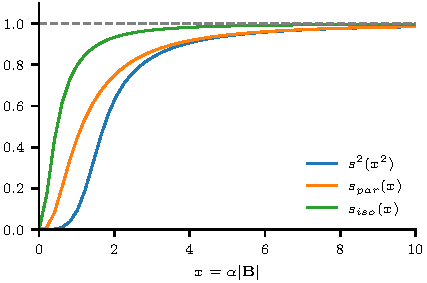
\includegraphics[width=0.5\linewidth]{alt_switching.pdf}
  \mycaption{Three potential switching functions.}{}%
  \label{fig:alt_switching}
\end{figure}

Figure~\ref{fig:alt_switching} plots the two Braginskii and the von Mises switching functions. The function $s_{par}$ shows the most similarity to the von Mises switching function, particularly the shallow slope near $|\vec{B}| = 0$, in contrast to the steeper slope of $s_{iso}$. Note that the argument of the von Mises switching function is the square of $x = \alpha |\vec{B}|$. This is a direct result of the choice of constitutive function $a(|\vec{B}|) = a_0 |\vec{B}|^2$, where $a_0 = \alpha^2$ for comparison.

\subsection{Calibrating the interpolation functions}

The parameters $a_0$ and $\alpha$ control the effective size of the isotropic region by controlling the degree to which the viscosity is anisotropic for a given field strength. From figure~\ref{fig:alt_switching}, the viscosity can be considered fully parallel when $\alpha |\vec{B}| = 10$. If the viscosity should be considered parallel when the field strength is some reference value $B_0$ then $\alpha = 10/B_0$ gives the appropriate parameter choice. Similarly, for the von Mises function, $a_0 = 100/B_0^2$. This calibration  can be seen in practice in the following example.

In the numerical experiments performed in chapter~\ref{chp:null_point_khi}, the magnetic field strength increases linearly with distance from the null point and the grid separation is found to be $\Delta x \approx 0.014$. If the viscosity is considered fully anisotropic at a radius of, say, ten grid points, the field at $x = 10 \Delta x$ is $|\vec{B}| = 0.14$, resulting in a calibrated $\alpha \approx 70$. The associated von Mises parameter would be $a_0 \approx 4900$. 

\section{Implementation of viscosity in Lare3d}

The two types of viscosity already present in the Lare3d code are shock and isotropic viscosities. Since shock viscosity is turned off for most numerical experiments presented in this thesis, I shall only detail the numerical implementation of isotropic viscosity, before discussing the implementations of the Braginskii and switching models.

\subsection{Review of the implementation of isotropic viscosity}

The isotropic viscous stress tensor is implemented in Lare3d as six 3D arrays, each storing the values for the six required components of a symmetric stress tensor. These are filled during the Lagrangian step using~\eqref{eq:isotropic_viscous_tensor}, where the components of the strain rate tensor are calculated via~\eqref{eq:rate_of_strain}. This stress tensor is used in the calculation of forces in the momentum equation and in the calculation of viscous heat contribution in the energy equation. This entire process is presented in detail below.

The strain rate tensor $\ten{W}$ is calculated in the code as
\begin{lstlisting}
sxx = (2.0_num * dvxdx - dvydy - dvzdz) * third
\end{lstlisting}
for the diagonal elements \verb|sxx|, \verb|syy| and \verb|szz| and
\begin{lstlisting}
sxy = (dvxdy + dvydx) * 0.5_num
\end{lstlisting}
for the off-diagonal elements \verb|sxy|, \verb|sxz| and \verb|syz|. Since $\ten{W}$ is a symmetric tensor, only six components need to be calculated. The gradients of velocity, written like \verb|dvxdy| for $\partial u_x / \partial y$, are calculated using finite differences between appropriate velocity components, where the velocity is interpolated between neighbouring grid points to ensure the resultant stress tensor is defined at the appropriate grid location. Note, the calculation of $\ten{W}$ in the code is a factor of a half smaller than the definition used in this thesis~\eqref{eq:rate_of_strain}. This is corrected for during the calculation of the viscous stress tensor, stored in the variable \verb|qxx|, where a factor of two is included,
\begin{lstlisting}
qxx(ix,iy,iz) = qxx(ix,iy,iz) + 2.0_num * sxx * rho(ix,iy,iz) * visc3
\end{lstlisting}
and similarly for the other five components of the tensor. The multiplication by \verb|rho| at this point is cancelled out at a later stage.

The gradient of the tensor is used in the calculation of the forces in the momentum equation in the following way. The tensor values must be averaged to ensure the resultant gradient is correctly aligned with the velocity grid locations. Similar calculations are carried out for the other components of the stress tensor and force vector. This same code is used to include the anisotropic viscous stress tensors when they are enabled.
\begin{lstlisting}
w1 = (qxx(ix ,iy ,iz ) + qxx(ix ,iyp,iz ) &
    + qxx(ix ,iy ,izp) + qxx(ix ,iyp,izp)) * 0.25_num
w2 = (qxx(ixp,iy ,iz ) + qxx(ixp,iyp,iz ) &
    + qxx(ixp,iy ,izp) + qxx(ixp,iyp,izp)) * 0.25_num
fx = fx + (w2 - w1) / dxc(ix)
\end{lstlisting}

The viscous heat is calculated using
\begin{lstlisting}
visc_heat(ix,iy,iz) = &
      qxy(ix,iy,iz) * dvxy  + qxz(ix,iy,iz) * dvxz &
    + qyz(ix,iy,iz) * dvyz  + qxx(ix,iy,iz) * dvxdx &
    + qyy(ix,iy,iz) * dvydy + qzz(ix,iy,iz) * dvzdz
\end{lstlisting}
and, just as in the calculation of the forces above, this same code is used to calculate the viscous heat generated by the anisotropic viscous tensors when they are enabled.

\subsection{Implementation of the Braginskii tensor}

Since the contribution of a generic viscous stress tensor to the momentum and energy equations is already included in the numerical implementation of isotropic viscosity, the only new piece of code required to implement a new stress tensor is the calculation of the stress tensor itself. The Braginskii tensor given by~\eqref{eq:brag_new} is implemented in the following way and, when enabled, replaces the calculation of the isotropic viscous stress tensor. 

The four coefficients of the terms in~\eqref{eq:brag_new} are calculated as
\begin{lstlisting}
a = (3._num*visc3 + brag_visc1 - 4._num*brag_visc2)&
    / MAX(2._num*mB2**2, none_zero)
b = (brag_visc1 - visc3)/(2._num*mB2)
c = (brag_visc2 - brag_visc1)/(mB2)
d = brag_visc1
\end{lstlisting}
where \verb|visc3| is the variable holding the value of $\eta_0$, \verb|brag_visc1| and \verb|brag_visc2| hold the values of $\eta_1$ and $\eta_2$, calculated via~\eqref{eq:perp_visc_coeff}, and \verb|mB2| holds the value of $|\vec{B}|^2$. The calculation of $\eta_1$ and $\eta_2$ is performed in the following way
\begin{lstlisting}
xi2 = (brag_alpha**2) * mB2
brag_visc_coeff = visc3*(6._num/5._num*xi2 + 2.23_num)&
                  / (2.23_num + 4.03_num*xi2 + xi2**2)
\end{lstlisting}
where \verb|brag_alpha| represents the parameter $\alpha$.

The quantity $(\ten{W} \vec{B}) \cdot \vec{B}$ and the tensor components of $\vec{B} \otimes \vec{B}$ are calculated using the following snippet.
\begin{lstlisting}
calc_wbdotb = 2._num*(&
  (bx*sxx + by*sxy + bz*sxz)*bx &
+ (bx*sxy + by*syy + bz*syz)*by &
+ (bx*sxz + by*syz + bz*szz)*bz)

btxx = bx**2
btyy = by**2
btzz = bz**2
btxy = bx*by
btxz = bx*bz
btyz = by*bz
\end{lstlisting}

This allows the Braginskii stress tensor to be calculated using
\begin{lstlisting}
bsxx = wbdotb*(a*btxx + b) + 2._num*d*sxx &
  + 4._num*c*(btxx*sxx + btxy*sxy + btxz*sxz)
\end{lstlisting}
and similar for the diagonal \verb|bsxx|, \verb|bsyy| and \verb|bszz| components. The off-diagonal components are calculated using the following snippet.
\begin{lstlisting}
bsxy = wbdotb*a*btxy + 2._num*d*sxy &
  + 2._num*c*(btxx* sxy + btxy* syy + btxz* syz &
            +  sxx*btxy +  sxy*btyy +  sxz*btyz)
\end{lstlisting}

Finally, the contribution from the Braginskii stress tensor is added to the total stress tensor using 
\begin{lstlisting}
qxx = qxx + rho*bsxx
\end{lstlisting}
and similar for the other components. A later calculation in Lare3d requires that the Braginskii stress tensor is multiplied by \verb|rho|. Since multiple separate stress tensors can be included, at this point in the execution \verb|qxx| may already contain a contribution from an unrelated tensor (such as shock viscosity), hence why \verb|bsxx| is added in this way. However, this is included for the benefit of other users of the code; in this thesis \verb|qxx| will only contain a single stress tensor: the isotropic stress tensor or one of the anisotropic stress tensors.

\subsection{Implementation of the switching model}

The numerical implementation of the switching model~\eqref{eq:switching_model} is similar to the implementation of the Braginskii model detailed previously, with the exception of the tensor itself which is calculated using
\begin{lstlisting}
bsxx = visc3*((1.0_num-s2)*sxx*2.0_num + 1.5_num*s2&
/MAX(mB2**2, none_zero)*wbdotb*(btxx - mB2*third))
\end{lstlisting}
where \verb|s2| holds the local value of the chosen switching function, and the diagonal \verb|bsxx|, \verb|bsyy| and \verb|bszz| components are calculated similarly. The off-diagonal components are calculated using the following snippet.
\begin{lstlisting}
bsxy = visc3*((1.0_num-s2)*sxy*2.0_num + 1.5_num*s2&
/MAX(mB2**2, none_zero)*wbdotb*(btxy))
\end{lstlisting}

As discussed in section~\ref{sec:switching_function}, the von Mises switching function $s^2$ is implemented as a spline approximation. The Braginskii switching functions~\eqref{eq:alt_switching1} and~\eqref{eq:alt_switching2} have been simplified using the Python package \emph{SymPy} and are implemented directly. 

\section{Application to stressed null point}

\label{sec:slow_null_point}

As a test of the switching model in a non-trivial topology, a series of simulations of magnetic null points subjected to twisting motions were carried out. Isotropic, Braginskii (without drift terms) and switching viscosity, with the three switching functions presented here, were used and the results compared. The shock viscosity was turned off in every experiment.

\subsection{Numerical setup}

The non-dimensionalised MHD equations are solved using the code Lare3d, introduced in chapter~\ref{chp:numerical_methods}. For the purposes of testing and comparing the various models, the typical values used to non-dimensionalise the MHD equations are arbitrary\footnote{For reference, the typical values are $B_0 = 0.03$ T, $L_0 = 180\times10^{3}$ m and $\rho_0 = 1.67\times10^{-4}$ kg m$^{-3}$, for the magnetic field strength, length and density, respectively.}. The domain is a cube of dimension $[-3, 3]^3$ and the resolution is $500$ or $100$ grid points per dimension. The magnetic field is initially prescribed as a linear magnetic null point,
\begin{equation}
  \label{eq:null_mag_field}
\vec{B} = (x, y, -2z)^T.
\end{equation}
The density $\rho$ is initially set to unity, the velocity to $\vec{u} = \vec{0}$, and the internal energy initially $\varepsilon = \gamma-1$, where $\gamma = 5/3$ is the specific heat ratio. Both viscosity and resistivity are uniform and take the value $\nu = \eta = 10^{-4}$.

On the lower boundary ($z=-3$) the velocity takes the form of a twisting vortex
\begin{equation}\label{ramp}
\boldsymbol{u} = \frac{v_0}{2}\left[1+\tanh\left(2\frac{t-t_0}{t_d}\right)\right]\boldsymbol{u}_h,
\end{equation}
with $\boldsymbol{u}_h = (u_x',u_y',0)^{\rm T}$ and
\begin{equation}\label{vprime}
u_x' = \left\{\begin{array}{cc}
-\pi y\displaystyle\frac{\sin(\pi r)}{r} &\quad{\rm if}\quad r^2<1, \\[8pt]
\displaystyle 0 &\quad{\rm if}\quad r^2 \ge 1,
\end{array}\right. \quad
u_y' = \left\{\begin{array}{cc}
\pi x\displaystyle\frac{\sin(\pi r)}{r} &\quad{\rm if}\quad r^2<1, \\[8pt]
\displaystyle 0 &\quad{\rm if}\quad r^2 \ge 1,
\end{array}\right.
\end{equation}
where $r^2=x^2+y^2$. On the opposite boundary, the twisting motion is reversed. The maximum driving velocity is set to $v_0 = 0.05$. The acceleration parameters are set to $t_0 = 2$, the time at which the velocity is half its maximum, and $t_d = 1$, resulting in maximum velocity being achieved around $t\approx4$. On the boundaries, all other variables keep their initial values and the derivatives through each boundary is zero.

For comparison between the switching models, the switching parameters are set to $\alpha = 6$ and $a_0 = \alpha^2 = 36$. This dramatically exaggerates the size of the isotropic region around the null point and allows good comparison of the viscosity models. These parameter choices result in the viscosity being nearly fully parallel at a distance of around $0.8$ from the centre of the null point. From the centre to this distance, the viscosity transitions from isotropic to fully parallel.

\subsection{Results}

\label{sec:slow_null_results}

The primary difference between isotropic and the anisotropic viscosity models is the magnitude and spatial distribution of the viscous heating. Isotropic viscosity overestimates the total heat generated by several orders of magnitude, when compared to any anisotropic model. The switching models all share some characteristics with the Braginskii model and each present different advantages.

\subsubsection{Differences in viscous heating rates}

\begin{table}[t]
  \centering
  \caption{Total heat generated up to $t=10$ by each model of viscosity for resolutions of $N=100$ and $500$.}
  \label{tab:slow_null_results_resolution}
  \begin{tabular}{c|ccccc}
Model &  Iso & Brag & Swi (von Mises) & Swi (par) & Swi (iso)\\
\midrule
$N=100$ &  $5.08 \times 10^{-3}$ & $5.74 \times 10^{-5}$ & $7.13 \times 10^{-5}$ & $8.39 \times 10^{-5}$ & $4.66 \times 10^{-5}$\\
$N=500$  &  $4.04 \times 10^{-3}$ & $5.25 \times 10^{-5}$ & $6.81 \times 10^{-5}$ & $7.80 \times 10^{-5}$ & $4.39 \times 10^{-5}$\end{tabular}
\end{table}

Table~\ref{tab:slow_null_results_resolution} shows the total heat generated by $t=10$ for each viscosity model for two different resolutions. The isotropic model overestimates the viscous heating by approximately two orders of magnitude compared to any of the anisotropic models. The switching models all dissipate similar amounts of heat to the Braginskii model, indicating that these models are approximating well the Braginskii tensor. The variance between each of the anisotropic models can be explained by considering how the isotropic and anisotropic parts of the tensors each contribute to the heating profile.

\begin{figure}[t]
    \centering
    \hfill
    \begin{subfigure}{0.32\textwidth}
      \includegraphics[width=1.0\linewidth]{iso_heating_iso_10.pdf}
      \caption{Isotropic}%
      \label{fig:iso_heating_iso_10}
    \end{subfigure}
    \hfill
    \begin{subfigure}{0.32\textwidth}
      \includegraphics[width=1.0\linewidth]{iso_heating_brag_10.pdf}
      \caption{Braginskii}%
      \label{fig:iso_heating_brag_10}
    \end{subfigure}
    \hfill
    \begin{subfigure}{0.32\textwidth}
      \includegraphics[width=1.0\linewidth]{iso_heating_switching_10.pdf}
      \caption{Switching (von Mises)}%
      \label{fig:iso_heating_switching_10}
    \end{subfigure}
    \begin{subfigure}{0.32\textwidth}
      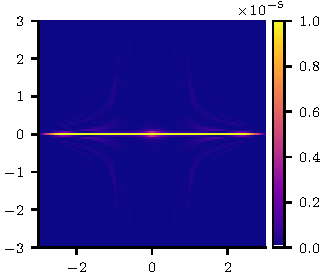
\includegraphics[width=1.0\linewidth]{iso_heating_switching2_10.pdf}
      \caption{Switching (par)}%
      \label{fig:iso_heating_switching2_10}
    \end{subfigure}
    \begin{subfigure}{0.32\textwidth}
      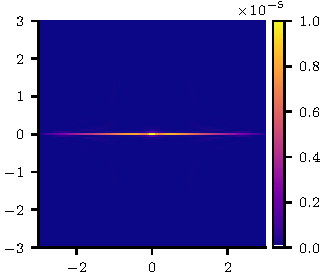
\includegraphics[width=1.0\linewidth]{iso_heating_switching3_10.pdf}
      \caption{Switching (iso)}%
      \label{fig:iso_heating_switching3_10}
    \end{subfigure}

    \mycaption{Isotropic heating generated by the viscosity models.}{Shown are plots of the isotropic heating produced by the isotropic, full Braginskii and switching models at $t=10$, sliced through $y=0$. Note the peak colour of the isotropic plot is an order of magnitude greater than that of the anisotropic models.}
\label{fig:isotropic_heating}%
\end{figure}

Figure~\ref{fig:isotropic_heating} shows the isotropic heating rate at time $t=10$ for each viscosity model. Isotropic viscosity heats at a generally greater rate than the anisotropic models, and the heating is distributed more extensively throughout the null. The boundary of the numerical cut-off, where isotropic viscosity turns off in the von Mises switching model, can be seen in figure~\ref{fig:iso_heating_switching_10}. The isotropic heating generated by the two Braginskii-inspired models show most similarity to that of the Braginskii model, with the isotropic-based switching model showing a nearly identical heating profile. This is to be expected since the coefficients of the isotropic contributions to the Braginskii and isotropic-based switching tensors are identical. The relative magnitude of the isotropic heating contributions for each anisotropic model reflects the total heat generated in table~\ref{tab:slow_null_results_resolution}, showing that the isotropic model overestimates viscous heating by two orders of magnitude.

Figure~\ref{fig:anisotropic_heating} shows the contributions to viscous heating from the anisotropic parts of the Braginskii and switching tensors. The anisotropic heating generated by the Braginskii tensor is dominated by the perpendicular contribution near the fan plane. This again reveals the potential issue with artificially increasing $\alpha$, that alongside increasing the size of the isotropic region, the extent of the perpendicular contributions are similarly enhanced.

While table~\ref{tab:slow_null_results_resolution} shows the global estimate of total viscous heat remains broadly consistent between different resolution for each of the viscosity models, figure~\ref{fig:anisotropic_heating} shows the spatial distribution of the heating does not. Figure~\ref{fig:anisotropy_bleeding} shows the heating rate produced by the anisotropic parts of the Braginskii and switching models and reveals the primary issue with the Braginskii model. When the resolution is too low to properly resolve the region around the null point, the Braginskii model erroneously heats anisotropically, primarily due to the artificially increased $\alpha$ enhancing the perpendicular components near the null point. This issue is mitigated by the switching models, all of which remove the perpendicular components of the Braginskii tensor. At the higher resolution of $N=500$ the von Mises switching model appears to remove more anisotropic heating than may be necessary however this could be solved by optimising the parameter $a_0$. Both Braginskii-based switching models show greater similarity to the Braginskii model without suffering from the issue of anisotropy at the null. Away from the null all switching models give similar results to the Braginskii model.

\section{Model efficiency}

In order to evaluate the computational efficiency of each model, a set of benchmark tests were run with the same physical setup as that of the test simulations found in section~\ref{sec:slow_null_point}, although changing the initial or boundary conditions should not affect the results. The resolution is set to $N=100$, all output is disabled, only one CPU core is used, and the simulations run for only $100$ timesteps. This number of timesteps allows the main loop of the simulation to run for a longer time than the overhead required to start and end the simulation, giving a more accurate estimate of the running time. The combination of the resolution and the number of timesteps results in the viscosity routines running $10^{8}$ times per simulation. The time is calculated via the Linux \verb|time| command which reports millisecond accuracy. Due to other software running on the same machine, the total time can vary. To measure a more accurate running time, the test for each model is repeated $25$ times and the results averaged. The machine used to run these tests is a Dell all-in-one with a 4 core, Intel i7-6700 CPU running at 3.4 GHz and the machine has 16 GB of RAM. 

\begin{figure}[t]
  \centering
  \includegraphics[width=0.5\linewidth]{benchmark.pdf}
  \mycaption{Relative computational efficiency of viscosity models measured via mean runtime.}{The runtime for each viscosity model is scaled by the runtime for the isotropic model.}%
  \label{fig:benchmark}
\end{figure}

Figure~\ref{fig:benchmark} shows the average runtime for each model. Since the isotropic model requires only the calculation of the rate of strain tensor, it is the quickest. The Braginskii model, being the most complex, requires many additional calculations to be carried out and this is reflected in its poorer runtime. The switching models show similar efficiencies, worse than the isotropic model but mostly better than the Braginskii model, as expected from considering the number of required calculations. The differences between the runtimes of the different interpolation functions are slight, although the von Mises implementation appears moderately faster. This is likely due to the spline representation of the von Mises function requiring only one computation of a cubic, while the other switching functions require two.

\section{Conclusion}

This chapter details the switching model, a new model of anisotropic viscosity specifically designed for use in numerical simulations of the solar corona. The model offers an alternative to the Braginskii model, capturing the main physics while avoiding the problem of anisotropic heating at the null point itself. It does this by artificially enlarging the isotropic region surrounding magnetic null points. The switching model does this by exposing a tunable interpolation function which measures the degree of anisotropy (dependent on the local magnetic field strength) and interpolates between isotropic and fully field-aligned viscosity. Three candidate interpolation functions are presented and their efficacy and computational efficiency compared. The switching model is generally found to be computationally more efficient than the Braginskii model and offers a good approximation to it.

Overall, the three switching functions behave similarly and each provide unique advantages. While the von Mises switching function is computationally faster than the Braginskii-inspired functions, it is a phenomenological model and requires a spline approximation for efficient implementation. In contrast, the Braginskii switching functions utilise the interpolation already implicit in the Braginskii tensor and can be implemented directly in the code. 

In chapters~\ref{chp:kink_instability} and~\ref{chp:kink_instability_straight} the von Mises switching model is employed although the field is strong enough everywhere that the tensor reduces to purely parallel (i.e. $\tilde{s} = 1$ everywhere). In chapter~\ref{chp:null_point_khi} the Braginskii-inspired parallel function~\eqref{eq:alt_switching1} is used to avoid the numerical cut-off associated with the spline representation.

\begin{figure}[t]
    \hfill
    \begin{subfigure}{0.49\textwidth}
      \includegraphics[width=1.0\linewidth]{aniso_heating_brag_10.pdf}
      \caption{Braginskii}%
      \label{fig:aniso_heating_brag_10}
    \end{subfigure}
    \hfill
    \begin{subfigure}{0.49\textwidth}
      \includegraphics[width=1.0\linewidth]{aniso_heating_switching_10.pdf}
      \caption{Switching (von Mises)}%
      \label{fig:aniso_heating_switching_10}
    \end{subfigure}
    \hfill
    \begin{subfigure}{0.49\textwidth}
      \includegraphics[width=1.0\linewidth]{aniso_heating_switching2_10.pdf}
      \caption{Switching (par)}%
      \label{fig:aniso_heating_switching2_10}
    \end{subfigure}
    \hfill
    \begin{subfigure}{0.49\textwidth}
      \includegraphics[width=1.0\linewidth]{aniso_heating_switching3_10.pdf}
      \caption{Switching (iso)}%
      \label{fig:aniso_heating_switching3_10}
    \end{subfigure}
    \mycaption{Anisotropic heating generated by the full Braginskii and switching models at time $t=10$.}{Close to the fan plane the Braginskii model shows notably greater anisotropic heating than any of the switching models. The switching models all appear similar though with minor differences near the null point.}
\label{fig:anisotropic_heating}%
\end{figure}

\begin{figure}[t]
    \hfill
    \begin{subfigure}{0.49\textwidth}
      \centering
      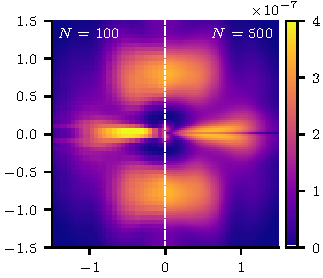
\includegraphics[width=1.0\linewidth]{diff_brag_resolution.pdf}
      \caption{Braginskii}%
      \label{fig:diff_brag_resolution}
    \end{subfigure}
    \hfill
    \begin{subfigure}{0.49\textwidth}
      \includegraphics[width=1.0\linewidth]{diff_switching_resolution.pdf}
      \caption{Switching (von Mises)}%
      \label{fig:diff_switching_resolution}
    \end{subfigure}
    \hfill
    \begin{subfigure}{0.49\textwidth}
      \includegraphics[width=1.0\linewidth]{diff_switching2_resolution.pdf}
      \caption{Switching (par)}%
      \label{fig:diff_switching2_resolution}
    \end{subfigure}
    \hfill
    \begin{subfigure}{0.49\textwidth}
      \includegraphics[width=1.0\linewidth]{diff_switching3_resolution.pdf}
      \caption{Switching (iso)}%
      \label{fig:diff_switching3_resolution}
    \end{subfigure}

    \mycaption{The effect of resolution on anisotropic heating rates.}{The anisotropic heating rate is plotted at resolutions of $100$ (left of each plot) and $500$ (right of each plot) grid points per dimension and both plots are slices through $x=0$ at $t=5$. When the null point is less resolved (left half of both figures) Braginskii viscosity erroneously permits anisotropic heating at the null. At higher resolutions (right half of both figures) the null is better resolved and much less anisotropic viscous heating is found at the null. All switching models avoid this issue.}
\label{fig:anisotropy_bleeding}%
\end{figure}
